\scanpage{155}
\[
\text{Conditions équivalentes :}\quad
\left\{\begin{aligned}
&\text{a) }\operatorname{Pic}^{0}_{C/k}\text{ est \unsure{abélien}}\\
&\text{b) les }\unsure{\kappa_{\alpha}|\mu_{\alpha}}=0\ \text{i.e. tous les pts doubles sont ordinaires,}\\
&\qquad\text{\uuline{et} }b_1=0\quad\text{[En particulier les }C_i\text{ sont non \unsure{singulières|singuliers}]}
\end{aligned}\right.
\]
\[
\text{Conditions équivalentes}\quad
\left\{\begin{aligned}
&\text{a) }\operatorname{Pic}^{0}_{C/k}\ \text{\unsure{n'a} pas de \unsure{composante} additive}\\
&\text{b) \deleted{\unsure{Pour|Donc}} }\unsure{\forall|\text{tt}}\,\alpha,\ \text{on a }\mu_{\alpha}=\unsure{\mu'_{\alpha}|\kappa'_{\alpha}}\\
&\qquad\text{i.e. le \unsure{recollement|conducteur} est trivial.}
\end{aligned}\right.
\]
\figure{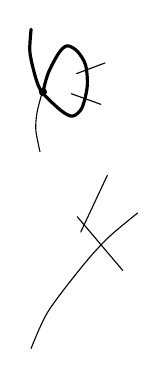
\begin{tikzpicture}[x=.0075cm,y=-.0075cm,line cap=round,line join=round]
\draw[line width=1.15pt] plot[smooth] coordinates {(84,518) (82,557) (92,601) (103,625) (134,655) (154,665) (170,651) (179,614) (176,578) (162,555) (145,546) (131,558) (113,592) (104,624)};
\draw plot[smooth] coordinates {(103,624) (94,659) (92,689) (99,725)};
\draw (161,593)--(209,575);
\draw (152,627)--(202,645);
\fill (104,624) circle[radius=.052cm];
\draw plot[smooth] coordinates {(84,1058) (113,995) (173,916) (215,870) (264,829)};
\draw (162,835)--(239,926);
\draw (168,861)--(213,765);
\end{tikzpicture}}
\[
\sum_i\nu_i=\underset{\mu_{\alpha}-1}{\sum_{\alpha}(\mu_{\alpha})}\deleted{\unsure{+1)|+1}}
=\underbrace{\sum_{\unsure{\beta|\rho}}(\deleted{\unsure{+}}\mu_{\alpha}-1)}_{c_0-1+\rho}+c_1
\]
\[
\deleted{\unsure{g=|g|\substack{3\\6}}}\qquad
\boxed{\sum\nu_i=c_0-1+\rho+c_1}
\]
\margin{$\rho=g-\sum g_i$\par $\sum g_i=g-\rho$}
\[
\begin{aligned}
&3g-\underbrace{3\rho-\unsure{3|2}c_0+\underset{\cdots}{\deleted{c_0}}-1+\rho}{}+c_1+\lambda\\
&3g-2\rho-2c_0+c_1+\lambda-1\\
&3g-3\quad \deleted{\unsure{=2c|=2}}\,[2(c_0+\rho)-c_1-\lambda-2]
\end{aligned}
\]
\figure{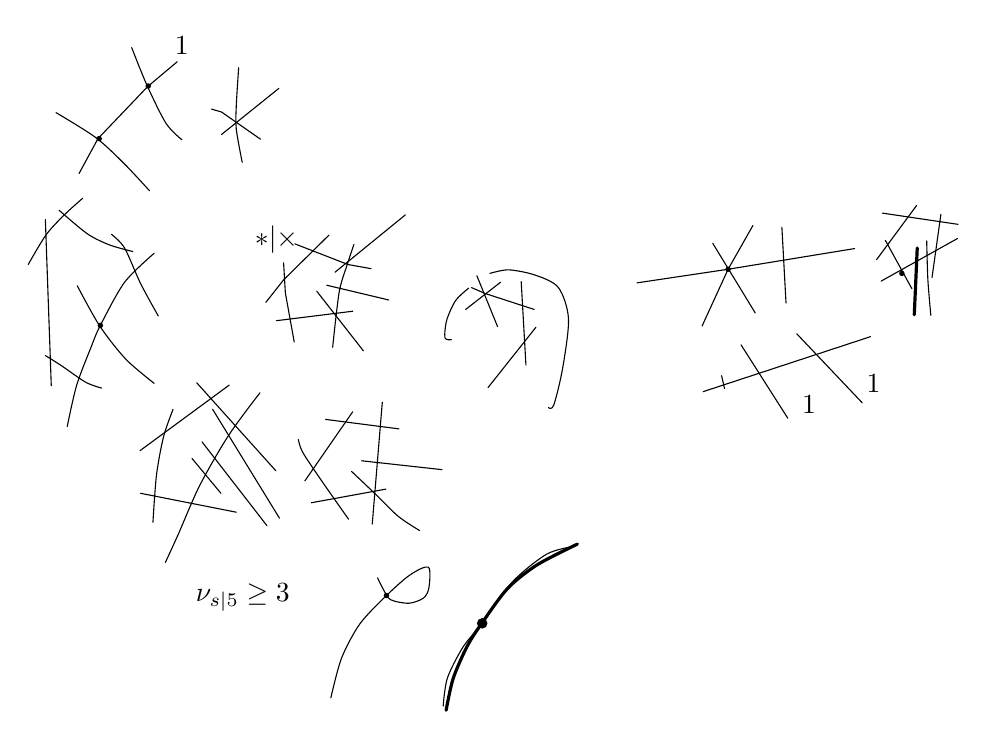
\begin{tikzpicture}[x=.0075cm,y=-.0075cm,line cap=round,line join=round]
\draw (144,1280)--(176,1221)--(260,1133)--(310,1091);
\draw plot[smooth] coordinates {(105,1177) (172,1219) (220,1263) (263,1309)};
\draw plot[smooth] coordinates {(233,1067) (259,1131) (291,1195) (318,1223)};
\node at (318,1064) {$1$};
\fill (178,1221) circle[radius=.035cm];
\fill (261,1132) circle[radius=.035cm];
\draw (368,1171)--(385,1176)--(451,1222);
\draw plot[smooth] coordinates {(414,1101) (410,1165) (410,1205) (420,1261)};
\draw (385,1214)--(482,1136);
\draw plot[smooth] coordinates {(58,1434) (88,1384) (119,1350) (150,1322)};
\draw plot[smooth] coordinates {(110,1342) (158,1382) (196,1401) (235,1412)};
\draw (87,1358)--(97,1639);
\draw plot[smooth] coordinates {(199,1383) (221,1406) (248,1466) (278,1521)};
\draw plot[smooth] coordinates {(124,1708) (140,1638) (165,1572) (180,1537) (221,1464) (271,1415)};
\draw plot[smooth] coordinates {(141,1470) (179,1538) (223,1594) (271,1635)};
\draw plot[smooth] coordinates {(87,1588) (114,1605) (155,1633) (182,1643)};
\fill (180,1537) circle[radius=.035cm];
\draw (460,1498)--(490,1460)--(567,1384);
\draw (490,1431)--(493,1482)--(508,1565);
\draw (509,1399)--(599,1434)--(638,1441);
\draw (577,1447)--(696,1350);
\draw plot[smooth] coordinates {(609,1400) (597,1436) (584,1481) (573,1574)};
\draw (563,1469)--(668,1494);
\draw (546,1479)--(625,1580);
\draw (478,1529)--(607,1513);
\node at (478,1392) {$\unsure{*|\times}$};
\draw plot[smooth] coordinates {(774,1561) (763,1558) (766,1528) (781,1495) (803,1474)};
\draw plot[smooth] coordinates {(839,1449) (871,1443) (916,1452) (955,1473) (972,1526) (962,1610) (947,1672) (938,1676)};
\draw (808,1473)--(831,1483)--(914,1510);
\draw (817,1453)--(852,1539);
\draw (798,1510)--(857,1464);
\draw (892,1463)--(900,1604);
\draw (836,1642)--(917,1540);
\draw (1088,1465)--(1242,1442)--(1456,1407);
\draw (1198,1538)--(1242,1442)--(1284,1368);
\draw (1216,1398)--(1288,1516);
\draw (1333,1371)--(1340,1499);
\fill (1242,1442) circle[radius=.035cm];
\draw (1493,1426)--(1561,1334);
\draw (1503,1347)--(1631,1366);
\draw (1508,1393)--(1553,1475);
\draw (1501,1462)--(1630,1390);
\draw (1602,1349)--(1587,1456);
\draw[line width=1.15pt] (1562,1406)--(1557,1519);
\draw plot[smooth] coordinates {(1578,1394) (1580,1460) (1585,1520)};
\fill (1536,1449) circle[radius=.035cm];
\draw (1200,1649)--(1483,1556);
\draw (1264,1570)--(1343,1694);
\draw (1358,1551)--(1469,1668);
\draw (1231,1622)--(1236,1644);
\node at (1379,1671) {$1$};
\node at (1488,1635) {$1$};
\draw (247,1749)--(398,1638);
\draw plot[smooth] coordinates {(269,1870) (275,1790) (287,1725) (303,1679)};
\draw (248,1821)--(410,1853);
\draw plot[smooth] coordinates {(290,1938) (312,1890) (348,1808) (397,1723) (450,1651)};
\draw (343,1634)--(477,1783);
\draw (370,1679)--(483,1863);
\draw (352,1734)--(462,1876);
\draw (335,1762)--(384,1821);
\draw (526,1800)--(607,1683);
\draw plot[smooth] coordinates {(515,1730) (522,1751) (551,1795) (600,1865)};
\draw (561,1696)--(685,1712);
\draw (657,1667)--(640,1873);
\draw (622,1766)--(758,1781);
\draw (537,1837)--(663,1814);
\draw plot[smooth] coordinates {(605,1784) (645,1822) (684,1860) (720,1884)};
\node at (421,1997) {$\nu_{\unsure{s|5}}\geq3$};
\draw plot[smooth] coordinates {(570,2167) (588,2100) (619,2042) (664,1994) (704,1959) (735,1946) (736,1980) (727,1998) (702,2007) (671,2001) (659,1984) (649,1964)};
\fill (664,1994) circle[radius=.035cm];
\draw[line width=1.15pt] plot[smooth] coordinates {(765,2188) (777,2134) (801,2079) (826,2040) (869,1982) (919,1942) (987,1907)};
\draw plot[smooth] coordinates {(760,2181) (767,2134) (793,2082) (824,2043) (877,1971) (935,1924) (980,1911)};
\fill (826,2041) circle[radius=.067cm];
\end{tikzpicture}}
Courbe elliptique $+k$ points dessus $(k\geq1)$.
\[
\unsure{k|R},\qquad 9-5=4
\]
\[
-6+2-1=-5
\]
% archive sheet number: 154
